\section{Preprocessing}
The bag of words model used by our classifiers is a good way to represent the data found in the given training documents. However this feature representation is prone to obtaining very high dimensions due to the large number of possible combinations that can be found in words. 

According to a recent survey performed by Google and Harvard, there are approximately 1,022,000 different words in the English language \cite{google2010words}. While we do not expect to find all possible words in the document corpus, a large number of them will be found along with their derivations in the form of spelling mistakes and grammatical variations (e.g.{\it they're} and {\it theyre}). Other non-English words such as html code, URLs and nonsensical data such as PGP keys will also be found within the documents.

Most of these words will provide no benefit to the classifier and in most cases will even harm the classifier's performance. It is therefore of utmost importance that noise in the text is filtered out and the number of word combinations is reduced to the most representative, yet minimal subset of the available words. The following steps are taken to do this:
\begin{itemize}
	\item Smart Email Parsing
	\item Simple Text Processing Techniques
	\item Stemming
	\item Feature Selection based on Document Frequency
\end{itemize}

Each of these steps contribute towards achieving a higher accuracy and performance in the classifier and will be described in detail in the sections below.

\subsection{Email Parsing}
\todo{This is our simple technique}
\todo{
    \begin{itemize}
        \item Strip metadata
        \item Strip HTML
        \item Multipart Splitting
    \end{itemize}
}
\todo{Improvement?}

\subsection{Stemming}
Most words in the English language are derived from a {\it morphological root} word that contains no prefixes or suffixes and conveys a very similar meaning to its derivation. A simple example of this is {\it subscriber} and {\it subscription} with their morphological root {\it subscribe}. 

If we can reduce all incoming words into their root form, we would be able to substantially reduce the number of dimensions for our model while also ensuring that words representing the same underlying feature are stored under the same value.

Unfortunately, such a task is quite hard and would probably require the creation of a very large lookup table for each word in the English language along with its root. This is due to the fact that the English language is not a formal language and hence does not follow a strict set of rules. 

We could however, take an approximation of the described process and instead derive the {\it stem} of each word. Like the morphological root, the stem is a representation of a words underlying meaning. However the stem does not guarantee to be a correct English word or generate the right root as its aim is simply to map variations of the same word to the same to item. 

For our Spam Filter implementation, we made use of the Porter Stemmer algorithm \cite{porter1980}, which in the authors words is ``a process for removing the commoner morphological and inflexional endings from words in English process''. In simpler terms, it is capable of removing known suffixes from words passed to it. The Porter Stemmer algorithm is available as open source code under the BSD License and is available in multiple languages, including Java which is made use of in our implementation.

Using the same examples shown before, passing {\it subscriber} and {\it subscribe} to the Porter Stemmer would reduce the words {\it subscribe} and {\it subscriber} to the stem {\it subscrib}. On the other hand, the word {\it subscription} will be wrongly mapped to a different stem - {\it subscript}. The latter is an example of where the approximation fails to produce the correct result, however in general most words passed to the algorithm have shown to produce favourable results.

In terms of the Spam Filter implementation, using Porter Stemming on the given set of training emails reduced the number of words from 24813 words to 18932 stems (both after text pre-processing). This is a substantial reduction in the number of dimensions and plays a crucial role in ensuring that the classifier is able to train with the given documents in a short amount of time and without requiring large amounts of memory. Apart from improving speed and reducing memory, it has also proved to improve classification performance. \todo{include some results - simple example I have is 0.973 with and 0.97 without}.

\todo{Improvement?}

\subsection{Feature selection}
\todo{Is this really preprocessing?}

As the number of features generated by the input data is even very high after the previous preprocessing steps, we are going to minimise its number by trimming features which are (significantly) relevant for the classification quality.

\todo{\dots}

\begin{figure}[h!]
    \centering
    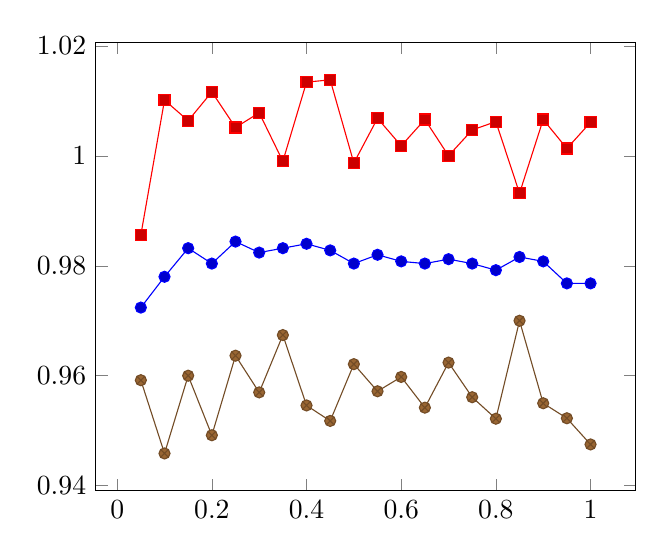
\begin{tikzpicture}
        \begin{axis}
             \addplot+[sharp plot] coordinates {
                (0.05, 0.972400)
                (0.10, 0.978000)
                (0.15, 0.983200)
                (0.20, 0.980400)
                (0.25, 0.984400)
                (0.30, 0.982400)
                (0.35, 0.983200)
                (0.40, 0.984000)
                (0.45, 0.982800)
                (0.50, 0.980400)
                (0.55, 0.982000)
                (0.60, 0.980800)
                (0.65, 0.980400)
                (0.70, 0.981200)
                (0.75, 0.980400)
                (0.80, 0.979200)
                (0.85, 0.981600)
                (0.90, 0.980800)
                (0.95, 0.976800)
                (1.00, 0.976800)
                };
             \addplot+[sharp plot] coordinates {
                (0.05, 0.972400+0.013206)
                (0.10, 0.978000+0.032125)
                (0.15, 0.983200+0.023186)
                (0.20, 0.980400+0.031215)
                (0.25, 0.984400+0.020746)
                (0.30, 0.982400+0.025424)
                (0.35, 0.983200+0.015799)
                (0.40, 0.984000+0.029394)
                (0.45, 0.982800+0.031010)
                (0.50, 0.980400+0.018287)
                (0.55, 0.982000+0.024819)
                (0.60, 0.980800+0.021014)
                (0.65, 0.980400+0.026199)
                (0.70, 0.981200+0.018804)
                (0.75, 0.980400+0.024298)
                (0.80, 0.979200+0.027011)
                (0.85, 0.981600+0.011593)
                (0.90, 0.980800+0.025799)
                (0.95, 0.976800+0.024528)
                (1.00, 0.976800+0.029285)
                };
             \addplot+[sharp plot] coordinates {
                (0.05, 0.972400-0.013206)
                (0.10, 0.978000-0.032125)
                (0.15, 0.983200-0.023186)
                (0.20, 0.980400-0.031215)
                (0.25, 0.984400-0.020746)
                (0.30, 0.982400-0.025424)
                (0.35, 0.983200-0.015799)
                (0.40, 0.984000-0.029394)
                (0.45, 0.982800-0.031010)
                (0.50, 0.980400-0.018287)
                (0.55, 0.982000-0.024819)
                (0.60, 0.980800-0.021014)
                (0.65, 0.980400-0.026199)
                (0.70, 0.981200-0.018804)
                (0.75, 0.980400-0.024298)
                (0.80, 0.979200-0.027011)
                (0.85, 0.981600-0.011593)
                (0.90, 0.980800-0.025799)
                (0.95, 0.976800-0.024528)
                (1.00, 0.976800-0.029285)
                };
    \end{axis}
    \end{tikzpicture}
    \caption{Accuracy w.r.t. upper threshold (lower threshold = 0)}
    \label{p:upperbound}
\end{figure}


